% =============================================================================
% Part 2: Background + The SLEEP Architecture
% =============================================================================

\section{Background}
\label{sec:background}

\paragraph{Synaptic tagging and capture.}
The synaptic tagging-and-capture (STC) hypothesis~\citep{frey1997synaptic,redondo2011making} posits that weak synaptic stimulation creates short-lived molecular ``tags'' which can later capture plasticity-related proteins (PRPs) synthesized in response to a separate strong stimulus, converting transient potentiation into durable change. STC explains how the brain implements selective consolidation: tags mark candidates, PRPs are the limited resource, and competition among tags determines which traces become permanent. Memory reconsolidation~\citep{nader2000fear} adds that previously consolidated traces become temporarily labile when re-accessed, allowing revision.

\paragraph{Complementary learning systems.}
Complementary Learning Systems (CLS) theory~\citep{mcclelland1995why} proposes two memory subsystems with distinct learning rates and storage formats: a fast hippocampal system that stores arbitrary episodic associations through one-shot binding, and a slow neocortical system that gradually accumulates statistical regularities. Sleep replay~\citep{wilson1994reactivation,diekelmann2010memory} bridges the two: the hippocampus reactivates recent experiences, training the neocortex while interleaving consolidated knowledge to prevent overwriting.

\paragraph{Parameter-efficient fine-tuning.}
Low-Rank Adaptation~\citep{hu2021lora} factors weight updates as $\Delta W = BA$ with $B \in \mathbb{R}^{d \times r}, A \in \mathbb{R}^{r \times d}$, $r \ll d$, training only $A,B$ while freezing the base model. LoRA enables targeted weight updates without full fine-tuning, making it the natural substrate for the slow consolidation system in our architecture.

\paragraph{Memory-augmented transformers.}
Standard transformer attention~\citep{vaswani2017attention} computes scores between learned queries and keys derived from the current context window. Memorizing Transformers~\citep{wu2022memorizing} augment this with a $k$-nearest-neighbor lookup over a bank of stored key-value pairs from past contexts. Schmidhuber's earlier fast-weight programmers~\citep{schmidhuber1992learning} proposed associative memory as outer-product weight updates. Both demonstrate that attention can be extended with external memory; both rely on retrieval-aware fine-tuning to teach the model to use that memory effectively. We adopt the KV-memory substrate from Memorizing Transformers but use it within a complete biologically-grounded consolidation pipeline rather than as a standalone retrieval mechanism.

\paragraph{Continual learning.}
Elastic Weight Consolidation~\citep{kirkpatrick2017overcoming} prevents forgetting by adding a Fisher-information-weighted quadratic penalty pulling parameters toward previous values. Generative replay~\citep{shin2017continual,rebuffi2017icarl} avoids storing raw old data by training a generator to synthesize old-task samples that are interleaved with new-task training. Both are mechanisms our consolidation step inherits.

\section{The SLEEP Architecture}
\label{sec:method}

SLEEP augments a frozen base model $W_{\mathrm{slow}}$ with three additions: (i) a \emph{tagging layer} that flags surprising spans during inference; (ii) a \emph{KV memory bank} (W$_{\mathrm{fast}}$) into which tagged spans are written one-shot; (iii) a \emph{consolidation adapter} (W$_{\mathrm{cons}}$, a LoRA module) that is updated during periodic ``sleep'' phases via replay-driven gradient descent under safety constraints. A \emph{PRP allocator} prioritizes which tags get consolidated. Figure~\ref{fig:architecture} summarizes the system.

\begin{figure}[h]
\centering
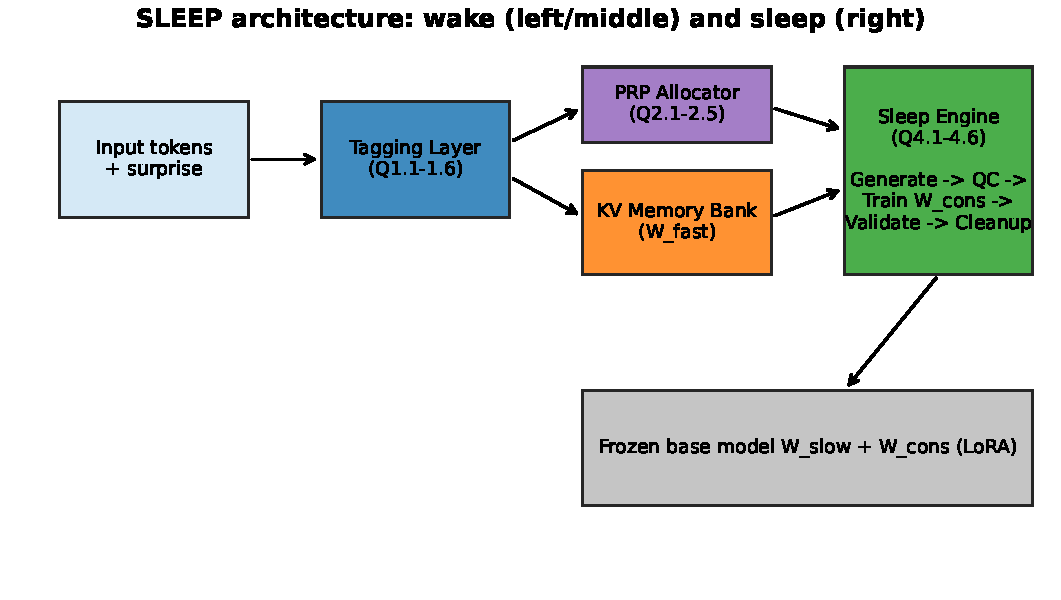
\includegraphics[width=0.95\textwidth]{figures/figure_architecture.pdf}
\caption{The SLEEP architecture (Figure~2; the paper's central \emph{empirical} result is on page~1, Figure~\ref{fig:pareto}). Wake phase: input tokens are processed by the tagging layer; tags allocate against the PRP budget and write episode-level K/V into the memory bank. Sleep phase: bank-conditioned generative replay produces synthetic training samples that drive gradient updates to W$_{\mathrm{cons}}$ under EWC + hard-clipping safety constraints. After successful consolidation, the bank is cleared.}
\label{fig:architecture}
\end{figure}

\subsection{Tagging Layer}
\label{sec:tagging}

For each input token $t$ at position $i$, the layer computes the model's per-token cross-entropy surprise $e_t = -\log p(x_t \mid x_{<t})$. An adaptive z-score thresholder maintains running mean $\mu$ and variance $\sigma^2$ via exponential moving average ($\beta = 0.99$) and flags positions where $(e_t - \mu)/\sigma > \kappa$ (default $\kappa = 1.5$). Adjacent flagged positions within $g = 3$ tokens are merged into spans; spans shorter than $4$ tokens are discarded. Each surviving span produces a \emph{tag} carrying a key vector $k = \mathrm{Proj}(\bar{h})$ derived from the mean hidden state, an initial strength $s_0 \propto \mathrm{tanh}(E_\mathrm{span} / \alpha)$, the source identifier, and the token range. Tags decay exponentially in time and are reinforced when accessed by similar future inputs (Q1.1--1.6 in the formalization).

\subsection{KV Memory (W$_{\mathrm{fast}}$)}
\label{sec:kv_memory}

A central design correction in this work is that \emph{tags are pointers, not storage}. The original formalization stored only the K and V projections of the tagged tokens themselves; in practice this captured isolated entity mentions (``Nimbus Holdings'') without their factual contents (revenue figures, dates). We replace this with \emph{episode-level} storage: when a tag fires, we extract pre-RoPE keys and raw values for the full sentence containing the tag from each adapted attention layer. Concretely, for adapted layer $\ell$:

\begin{equation}
    K^{(\ell)}_{\mathrm{mem}} = W^{(\ell)}_K \cdot \mathrm{LayerNorm}_\ell(h^{(\ell)}_{\mathrm{episode}}), \quad V^{(\ell)}_{\mathrm{mem}} = W^{(\ell)}_V \cdot \mathrm{LayerNorm}_\ell(h^{(\ell)}_{\mathrm{episode}}),
\end{equation}

where $h^{(\ell)}_{\mathrm{episode}}$ is the input hidden state at layer $\ell$ across the full episode, captured via \texttt{output\_hidden\_states=True}. Crucially, the layer-norm is applied before the projections to match what the model computes during its own attention forward---without this correction, extracted K/V differ from in-attention K/V by exactly one normalization, producing silently wrong attention scores.

At inference, stored K/V are injected as a prefix at \emph{negative position IDs} $[-n_\mathrm{mem}, -1]$ in each adapted layer's attention. RoPE~\citep{su2024roformer} is applied to memory keys at read time; because RoPE is a relative-position rotation, the memory at negative positions appears to current queries as ``recent prefix tokens,'' a regime the model was trained to handle. Per-query top-$k$ retrieval gating~\citep{wu2022memorizing} restricts attention to the $k$ memory positions whose Q$\cdot$K inner product is highest, with gating implemented through a $-\infty$ additive mask on excluded positions in the model's existing attention machinery.

The bank is per-tag indexed and supports per-tag eviction. Capacity is bounded by total stored tokens; capacity policy is delegated to the PRP allocator.

\subsection{PRP Allocation}
\label{sec:prp}

A composite score combines four signals (Q2.1 in the formalization):

\begin{equation}
    \mathrm{score}(\tau) = w_1 \cdot E_{\mathrm{span}}^{\mathrm{norm}} + w_2 \cdot \mathrm{access}^{\mathrm{norm}} + w_3 \cdot \mathrm{xref} + w_4 \cdot e^{-\Delta t / \tau_r},
\end{equation}

with weights $(0.35, 0.30, 0.15, 0.20)$. Cross-reference density $\mathrm{xref}$ measures how many other tags have similar keys (cosine similarity $> 0.5$). PRP allocation is competitive: only tags whose score exceeds an adaptive threshold $\theta_{\mathrm{prp}}$ receive an allocation token $p = 1$, and the budget $B = c_{\mathrm{prp}} \cdot N_{\mathrm{params}}^{(B)}$ caps the total. Allocated tags become candidates for sleep consolidation.

\subsection{Sleep Engine}
\label{sec:sleep_engine}

A sleep cycle proceeds in five phases, with KV memory injection enabled or disabled per phase to enforce intended semantics:

\begin{enumerate}[itemsep=0.15em,topsep=0.2em]
    \item \textbf{Generate} (KV active). For each candidate tag, produce a replay sample by autoregressively sampling from the model conditioned on the early tokens of the source episode. With KV memory active, the model can attend to the original experience while compressing it.
    \item \textbf{Quality check}. Replays are retained if (a) cosine similarity to the source $> 0.5$ and (b) mean per-token surprise exceeds a calibration threshold $\mu_{\mathrm{surprise}}$.
    \item \textbf{Train} (KV disabled). W$_{\mathrm{cons}}$ is updated by gradient descent on the accepted replays interleaved 1:1 with self-generated samples drawn from the unadapted base model (the ``old knowledge'' arm). Training disables KV injection so that W$_{\mathrm{cons}}$ learns to encode the replay content into weights rather than relying on the bank as a crutch.
    \item \textbf{PPL check} (optional, KV disabled). On benchmark data, post-training perplexity is compared to pre-training. If degradation exceeds $\epsilon_{\mathrm{degrade}}$, W$_{\mathrm{cons}}$ is rolled back.
    \item \textbf{Validate \& cleanup} (KV disabled). For each candidate tag, the post-training model's surprise on the original span is compared to the pre-training surprise; passes if the reduction is at least $\epsilon_{\mathrm{learn}}$ (default 10\%). Passing tags are removed from the buffer; failing tags are penalized; tags that fail repeatedly are evicted permanently.
\end{enumerate}

After successful consolidation, the KV bank is cleared---its content has (in principle) transferred to W$_{\mathrm{cons}}$.

\subsection{Safety Machinery}
\label{sec:safety}

W$_{\mathrm{cons}}$ training applies four safety mechanisms simultaneously:

\textbf{EWC penalty}~\citep{kirkpatrick2017overcoming}: a Fisher-weighted quadratic regularizer pulls W$_{\mathrm{cons}}$ toward its pre-training checkpoint, with strength $\lambda_{\mathrm{EWC}}$ (default 100).

\textbf{Hard clipping}: after each optimizer step, per-parameter changes are clipped to magnitude $\delta_{\max}$ (default 0.01) relative to the pre-cycle checkpoint, and gradients are scaled by per-layer plasticity coefficients $\phi_\ell \in [\phi_{\min}, 1]$ encoding ``hippocampal-like'' top-third layers as more plastic.

\textbf{Old-knowledge interleaving}: each training step mixes replay samples with self-generated continuations from the unadapted base model, providing a regularization pressure toward preserving base capabilities.

\textbf{Validation rollback}: candidates whose surprise on the original span does not drop by $\epsilon_{\mathrm{learn}} = 0.10$ are rolled back to their pre-cycle parameter values.

The cumulative effect is a strong stability bias. The empirical question is whether this bias is correctly calibrated. Section~\ref{sec:results} shows it is not, in single-cycle settings; Section~\ref{sec:multi_cycle} shows it is more justified in multi-cycle settings.
